\DiaryEntry{Markov Chains, 1}{2019-02-07}{Stochastic}

\subsection{Introduction}

A Markov process is a special type of stochastic process. We concentrate on discrete time processes; in this context a random process is a family of random variables $\{X(t), t=0,1,2,\ldots \}$. For a discrete-time random process to have the Markov property, it must fulfill,

\bee
P(X_{n+1}=x_{n+1} | X_n = x_n, X_{n-1} = x_{n-1}, \ldots, X_0 = x_0) = P(X_{n+1}=x_{n+1} | X_n = x_n)
\eee

I.e. the probability for state $n+1$ depends only on state $n$ and not on previous states. The probabilities $P(X_{n+1}=x_{n+1} | X_n = x_n)$ are denoted single-step transition probabilities and will be denoted as

\bee
P(X_{n+1}=j | X_n = i) = p_{ij}(n)
\eee

The indices go from ``previous to current'' state. Note also that the transition probabilites may depend on absolute time $n$ (inhomogenous Markov chain). We can collect the transition probabilites into a matrix as follows

\bee
P = \begin{bmatrix} p_{00}(n) & p_{01}(n) & \cdots & p_{0j} & \cdots \\
  p_{10}(n) & p_{11}(n) & \cdots & p_{1j} & \cdots \\
  \cdots \\
  p_{i0}(n) & p_{i1}(n) & \cdots & p_{ij} & \cdots \\
\end{bmatrix}
\eee

Note that all matrix entries must be positive and all rows must sum to one; i.e. $\sum_j pij(n)=1$. A matrix fulfilling these conditions is called a Markov matrix or stochastic matrix.

In the following we will concentrate on homogenous Markov chains.


\paragraph{Example.} In the following example, we have three states $1,2,3$ each having transition probabilities as shown in the Figure. 


\begin{figure}[H]
  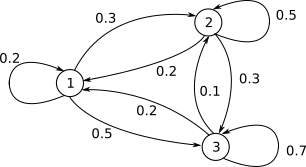
\includegraphics[scale=1.0]{images/markov_1_1.png}
\end{figure}

The corresponding transition probability matrix is therefore

\bee
P = \begin{bmatrix} 0.2 & 0.3 & 0.5 \\
  0.2 & 0.5 & 0.3 \\
  0.2 & 0.1 & 0.7
  \end{bmatrix}
\eee

\subsection{Chapman-Kolmogorov Equations}

A sequence of states visited by the chain is called a sample path. The probability for a sample path is given as follows

\bee
P(X_{n+m}=a, X_{n+m-1}=b, \ldots, X_{n+1}=j | X_n = i) = p_{ij}p_{jk}\cdots p_{cb}p_{ba}
\eee

We next restrict to the probability of sample paths with defined length, ending in state $k$ and starting in state $i$. As an example consider length $2$. Then the probability for a specific sample path (going via state $j$) is

\bee
P(X_{2}=k, X_{1}=j | X_{0}=i) = p_{ij}p_{jk}
\eee

If we want the probility $p_{ik}^{(2)}$ of all sample paths with length $2$, starting in $i$ and ending in $k$, we need to sum over all states in between; i.e.

\bee
p_{ik}^{(2)} = \sum_j P(X_{2}=k, X_{1}=j | X_{0}=i) = \sum_j p_{ij}p_{jk}
\eee

We can extend this to longer sample paths in an inductive manner

\bee
p_{il}^{(3)} = \sum_j \sum_k p_{ij}p_{jk}p_{kl} = \sum_j p_{ij} p_{jl}^{(2)}
\eee

We can collect the $p_{ik}^{(2)}$ in a matrix $P^{(2)}$ which is connected to $P$ via

\bee
P^{(2)} = P^2
\eee

Here the summation across the nodes in between is done implicitely by the matrix multiplication. Of course, this generalizes to longer paths as

\bee
P^{(N)} = P^N
\eee

Let $\pi^{(n)}$ denote the row vector containing probabilities for the states at time $n$, we have

\bee
\pi^{(1)} = \pi^{(0)} P
\eee

Note that we need to multiply the vector from the left with the matrix. By an induction argument we can extend this to

\bee
\pi^{(N)} = \pi^{(0)} P^N
\eee

We can take the limit $\lim_{N \rightarrow \infty} P^N$ and in some cases the limit exists and all rows are the same. This shows that $\pi^{(N)}$ becomes independent of the initial state. In our example the limit exists and equals

\bee
\lim_{N \rightarorrw \infty} P^N = \begin{bmatrix}
0.2  & 0.233351  & 0.566649 \\
0.2  & 0.233351  & 0.566649 \\
0.2  & 0.233351  & 0.566649
\end{bmatrix}
\eee

\subsection{State Classification}


%%% Local Variables:
%%% mode: latex
%%% TeX-master: "journal"
%%% End:
